%%%%%%%%%%%
% METHODS %
%%%%%%%%%%%

\section{Clustering and Softmax Distance as a Confidence Metric}

%\subsection{Clustering and Softmax Distance Threshold}

We consider a neural network output vector $\mathbf{p} = (p_1, p_2, \dots, p_K)$ where $\sum p_i = 1$, representing a probability distribution obtained by normalizing the logit vector $\mathbf{z} = (z_1, z_2, \dots, z_K)$ through the softmax function, $p_i = \text{softmax}(z_i) = e^{z_i} / \sum_{j=1}^{K} e^{z_j}$. For example, given $\mathbf{p} = [0.01, 0.01, 0.01, 0.01, 0.9, 0.01, 0.01, 0.01, 0.01, 0.01]$, the predicted class is '4', corresponding to the highest value at index five, reflecting the confidence of the prediction for each class from '0' to '9'. The logits, representing log-likelihoods of class memberships, are related to probabilities by $z_i = \log (p_i / (1 - p_i))$ where $z_i$ is the logit for class $i$, and $p_i$ is the probability of the input belonging to class $i$\cite{goodfellow2016deep, bishop2006pattern}.

We store the predictions for MNIST and CIFAR-10 datasets in a matrix $\mathbf{M} \in \mathbb{R}^{n \times 12}$, where $n$ is the number of predictions, the first ten columns are the softmax probabilities, column 11 is the true class and column 12 is the predicted class.

To obtain cluster centroids $\mathbf{C} \in \mathbb{R}^{10 \times 10}$ we calculate the mean of all correct predictions from the training datasets with Algorithm \ref{alg:k-means-centroid-init}. To calculate the softmax distance threshold we use all incorrect predictions with Algorithm \ref{alg:min_distance}.

\begin{algorithm}
\caption{K-Means Centroid Initialisation from Softmax Outputs}
\label{alg:k-means-centroid-init} 
\begin{algorithmic}[1]
\Require{$correct\_preds$: array of shape $(n, 12)$, where $n$ is the number of correct predictions}
\Ensure{$centroids$: array of shape $(10, 10)$, initialised centroids for each digit class}

\State $probs\_dist \gets corrects\_preds[:, :10]$ \Comment{Extract probability distribution for each digit}
\State $centroids \gets \text{zeros}((10, 10))$ \Comment{Initialise centroids array}

\For{$digit \gets 0$ to $9$}
\State $indices \gets \text{where}(\text{argmax}(probs\_dist, \text{axis}=1) == digit)[0]$ \Comment{Find indices of rows where digit has highest probability}
\State $centroid \gets \text{mean}(probs\_dist[indices], \text{axis}=0)$ \Comment{Compute mean probability distribution for selected rows}
\State $centroids[digit] \gets centroid$ \Comment{Assign centroid to corresponding row in centroids array}
\EndFor

\State \textbf{return} $centroids$
\end{algorithmic}
\end{algorithm}


%\subsection{Neural Networks}

% Moved from Methods to better spread out figures
\begin{figure*}[ht]
    \centering
    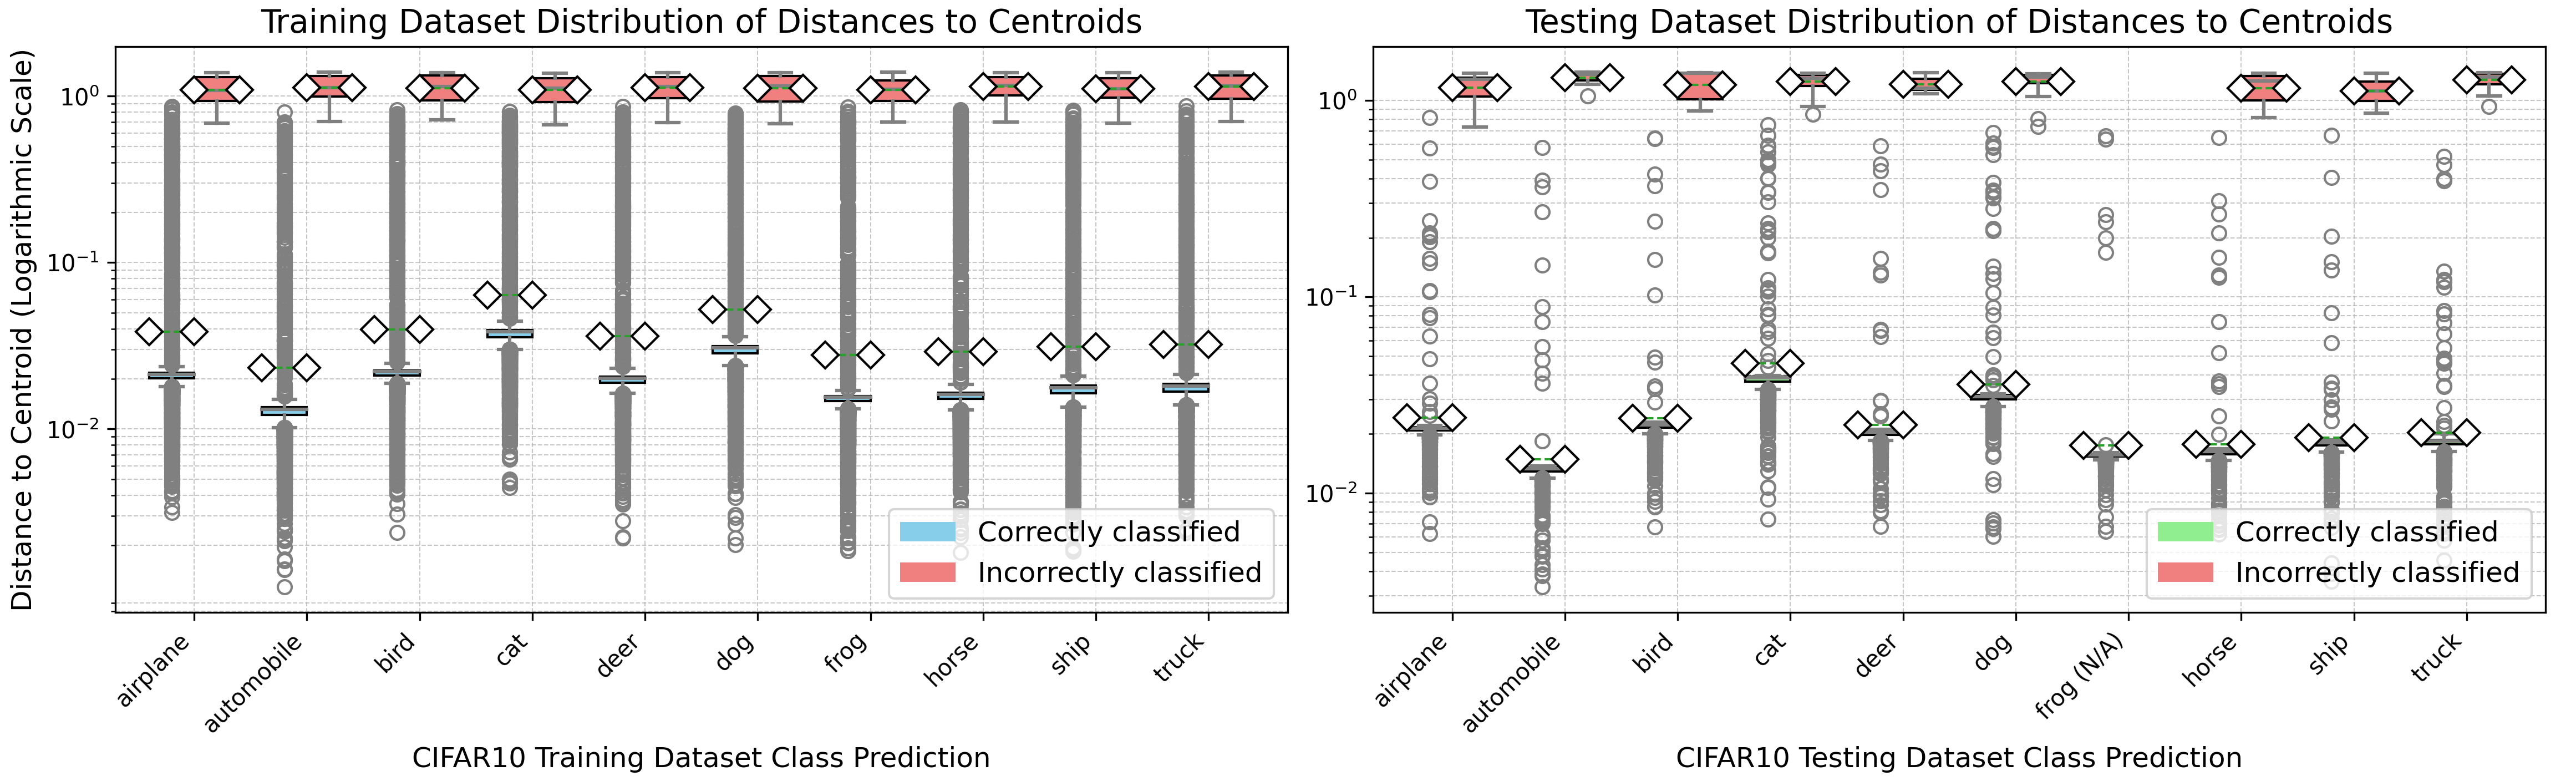
\includegraphics[width=0.99\textwidth]{Figures/CIFAR10_boxplots_side_by_side_x2.png}   \captionsetup{justification=raggedright,singlelinecheck=false}
    \caption{Distribution of Distances to Centroids for Correctly and Incorrectly Classified Instances in Training and Testing CIFAR-10 data, where training data is on the left and testing data is displayed on the right. Distances on y axis are shown on a logarithmic scale. Centroids are obtained from correctly classified training examples, then used for both training and testing datasets, a cluster is not created from the testing softmax distances. On the testing dataset, no frogs as misclassified, hence the missing top bloxplot. The corresponding plot for the MNIST dataset results is given in the supplementary materials.}
    \label{fig:CIFAR10_boxplots_side_by_side_x2}
\end{figure*}

% MNIST CNN

\textbf{Convolutional Neural Network}: A Convolutional Neural Network (CNN) is used to classify handwritten digits from the MNIST dataset, consisting of 60,000 training images and 10,000 testing images, each of size 28x28 grayscale (single channel) pixels, representing digits from 0 to 9.

The CNN architecture, implemented using PyTorch, consists of two convolutional layers followed by two fully connected layers. The first convolutional layer has 16 filters with a kernel size of 3x3 and a padding of 1. The second convolutional layer has 32 filters with the same kernel size and padding. Each convolutional layer is followed by a ReLU activation function and a max-pooling layer with a pool size of 2x2. The output of the second convolutional layer is flattened and passed through two fully connected layers with 128 and 10 neurons, respectively. The final output is passed through a log-softmax function to obtain the predicted class probabilities.
\begin{algorithm}
\caption{Find Minimum Softmax Distances to Centroids for Incorrectly Predicted Digits (Threshold)}
\label{alg:min_distance} 
\begin{algorithmic}[1]
\Procedure{FindMinDistances}{$data$}
    \State $labels \gets [0, 1, 2, 3, 4, 5, 6, 7, 8, 9]$
    \State $thresh \gets \text{empty array of shape } (10, 2)$
    \For{$i \gets 0 \text{ to } 9$}
        \State $label \gets labels[i]$
        \State $min\_dist \gets \min(data[data[:, 1] == label, 0])$
        \State $thresh[i, 0] \gets min\_dist$
        \State $thresh[i, 1] \gets label$
    \EndFor
    \State \textbf{return} $thresh$
\EndProcedure
\end{algorithmic}
\end{algorithm}
The model was trained using the Stochastic Gradient Descent (SGD) optimizer with a learning rate of 0.01 and a batch size of 64. The learning rate was determined using a custom learning rate function that decreases the learning rate over time. The Cross-Entropy Loss function was used as the criterion for optimization. The model was trained for 10 epochs.

The MNIST dataset was preprocessed using a transformation pipeline that converted the images to PyTorch tensors and normalized the pixel values to have a mean of 0.5 and a standard deviation of 0.5. The dataset was then loaded using PyTorch's DataLoader, for batch processing and shuffling of the data.

The total number of parameters for the MNIST classification CNN is 206,922 and took 5m6s to train on a Dell Precision Tower 5810 with a 6 core Intel Xeon Processor and 32GB memory running Ubuntu 18.04.  
%%%%%%%%%%%%%%%%%%%%
% NETWORK TRAINING %
%%%%%%%%%%%%%%%%%%%%
% Training time
The CNN/MNIST classifier took 5m6s to train. The accuracy on the training dataset is 98.38\% and 98.46\% on the testing dataset. 


\textbf{Vision Transformer}: The Vision Transformer (ViT) architecture \cite{dosovitskiy2020image} is implemented using the Hugging Face Transformers \cite{wolf2020huggingfaces}
library. The model used in this study, 'google/vit-base-patch16-224-in21k' \cite{wu2020visual}, is pre-trained on the ImageNet-21k dataset \cite{deng2009imagenet}, which contains 14 million labeled images. The pre-trained model is then fine-tuned on the CIFAR-10 dataset.
The ViT model divides an input image into patches and processes them using a Transformer encoder. The model used in this study has a patch size of 16x16 and an image size of 224x224. The ViT model outputs a representation of the image, which is then passed through a linear layer to obtain the final class probabilities.
The model has 86.4M parameters and is fine-tuned to classify images from the CIFAR-10 dataset, consisting of 50,000 training images and 10,000 testing images, each of size 32x32 pixels, representing 10 different classes: airplane, automobile, bird, cat, deer, dog, frog, horse, ship, and truck.

The data preprocessing pipeline involves on-the-fly data augmentation using the torchvision library's transforms module. The training data undergoes random resized cropping, random horizontal flipping, conversion to a tensor, and normalization. The validation and testing data are resized, center-cropped, converted to a tensor, and normalized.

The model is trained using the Hugging Face Trainer API. The learning rate is set to $2 \times 10^{-5}$, the per-device train batch size is 10, the per-device eval batch size is 4, and the number of training epochs is 3. The weight decay is set to 0.01. The model is trained on Google Colab Pro, T4 GPU hardware accelerator with high ram. The ViT/CIFAR-10 classifier took 1h15m to train, registering 99.04\% accuracy on the testing dataset.

% Moved from Results for a better spread of images

\begin{figure*}[ht]
    \centering
    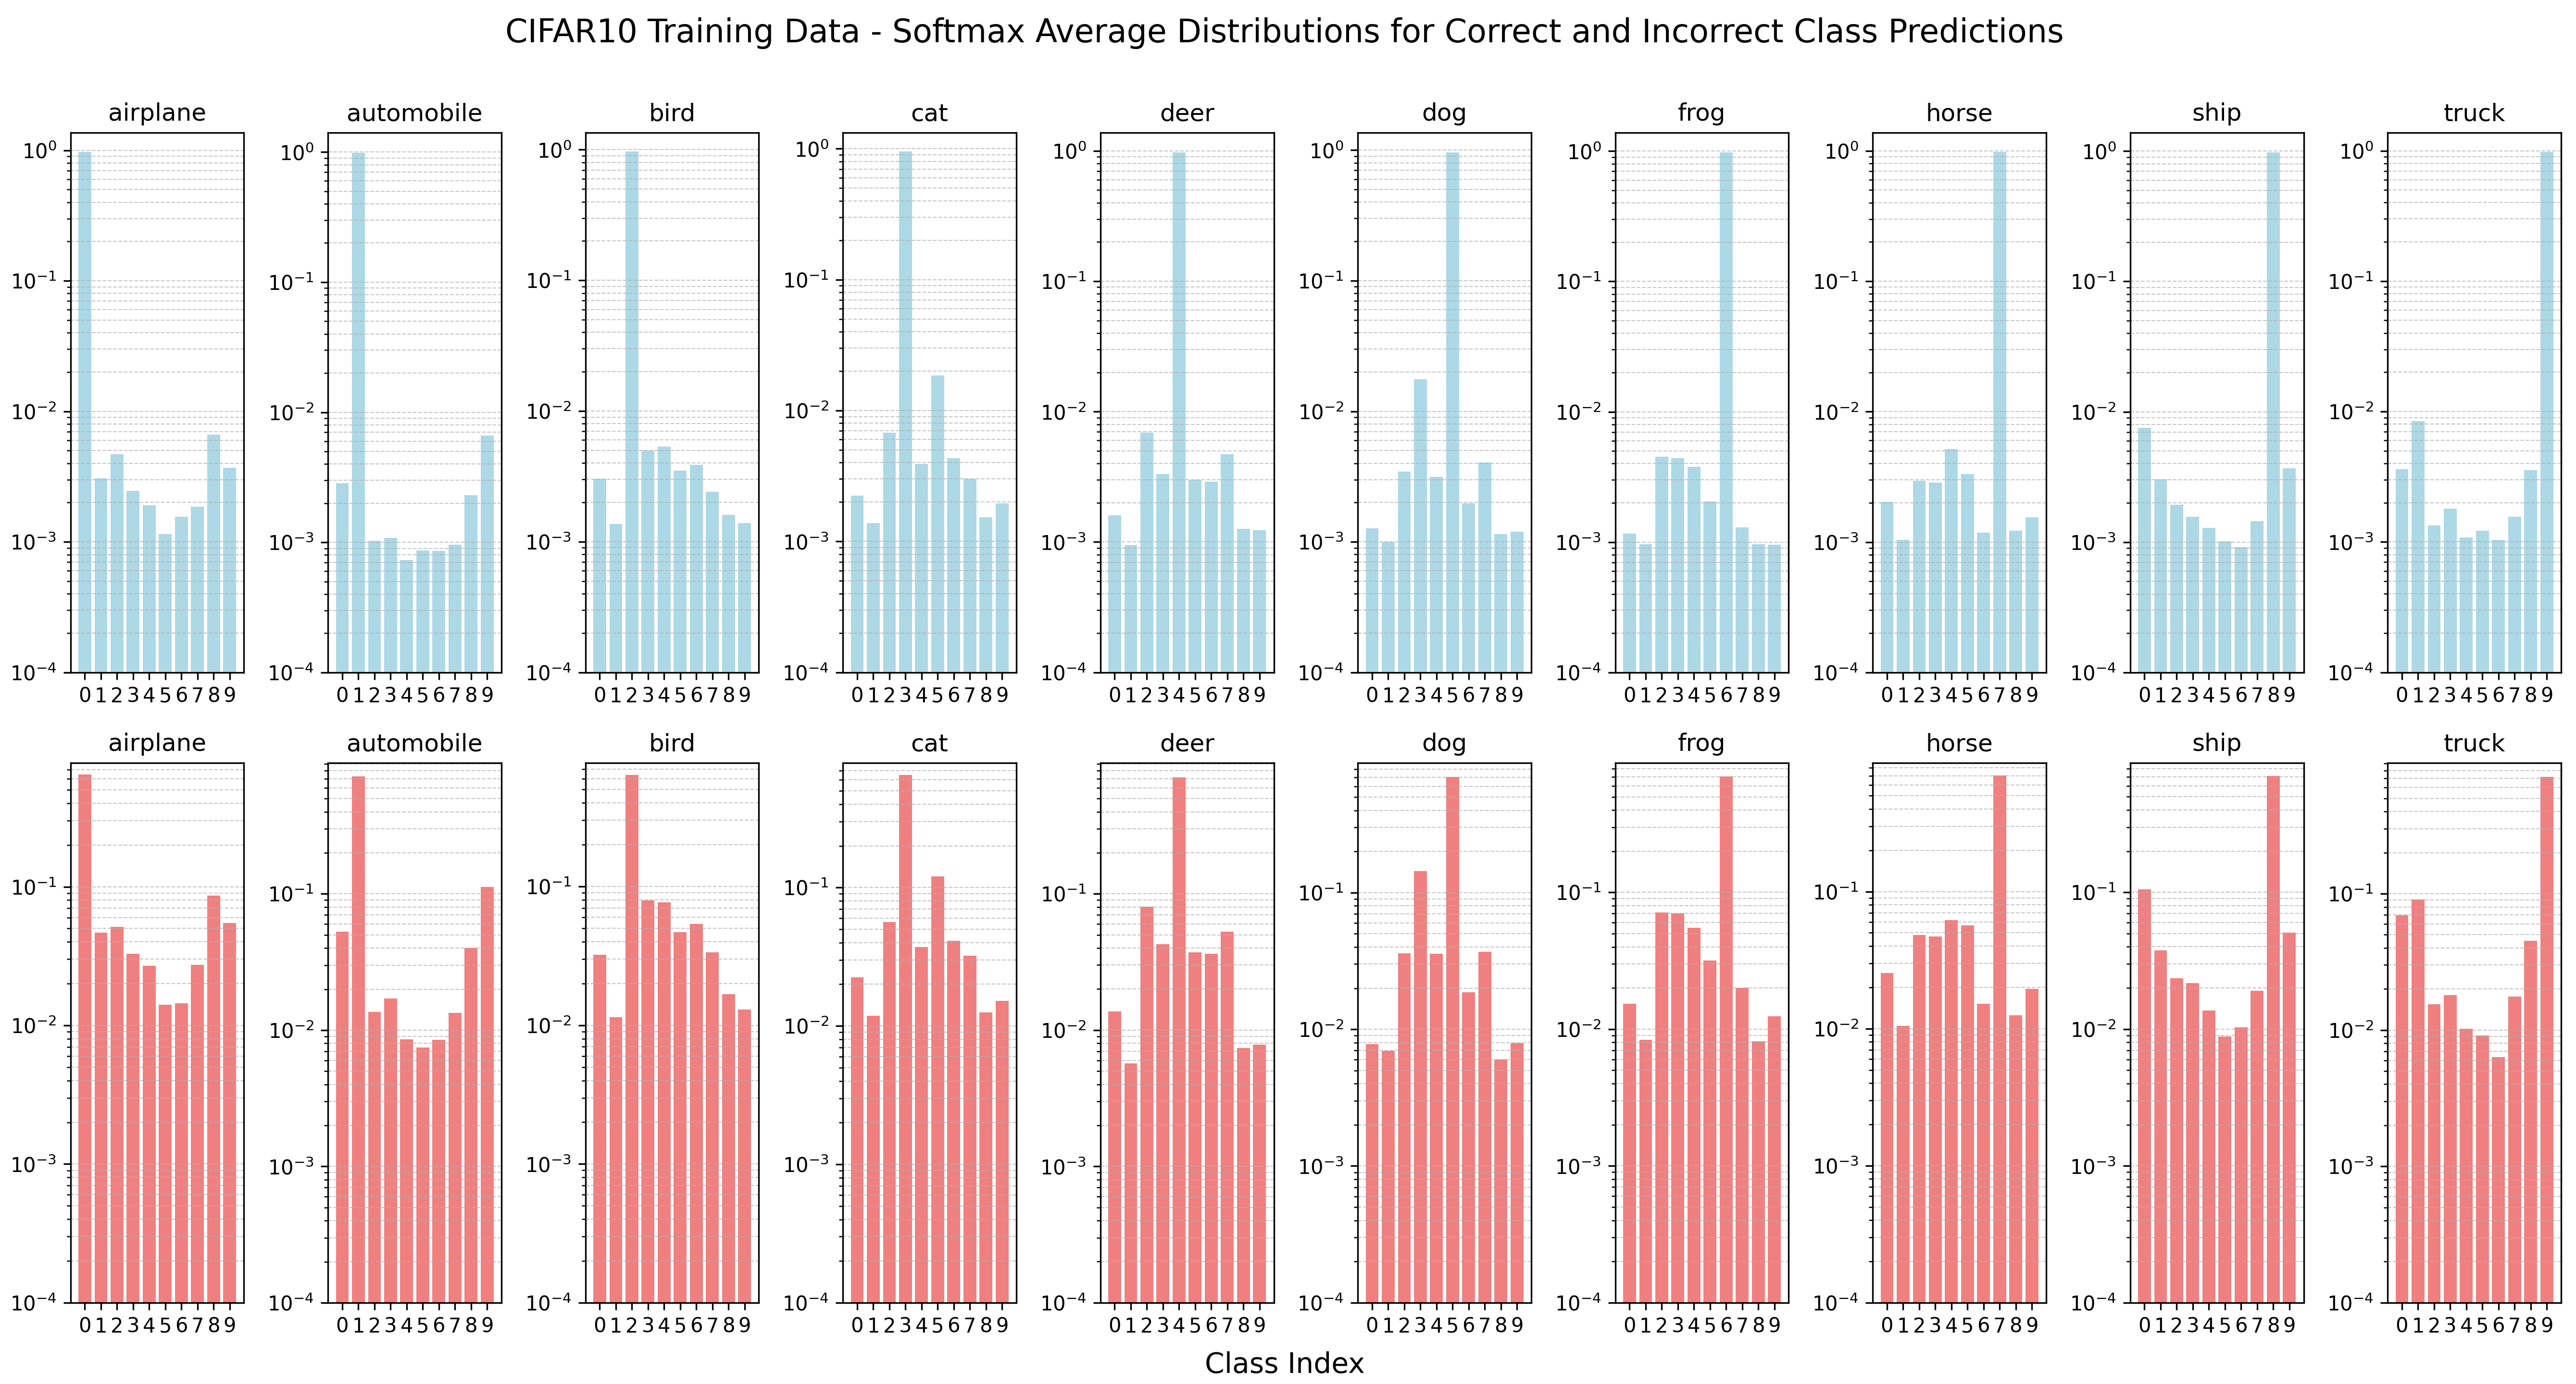
\includegraphics[width=0.99\textwidth]{Figures/CIFAR10_training_plot_centroid_distance_bars.png}
    \caption{Average Softmax Probabilities for ViT Correctly and Incorrectly Classified Classes in the CIFAR-10 Training Dataset. The ViT/CIFAR-10 testing dataset, and CNN/MNIST training and testing dataset equivalent results are given in the supplementary materials.}
    \label{fig:CIFAR10_training_plot_centroid_distance_bars.png}
\end{figure*}